\documentclass[usenames,dvipsnames]{beamer} %

%%%BASICS
\usepackage{xcolor}  % Colored tables
\usepackage{colortbl}  % Colored tables
\usepackage[utf8]{inputenc}
\usepackage{csquotes}

%%%START THEME SETTINGS
\usetheme{Madrid}
% \usecolortheme{beaver}
\useoutertheme{infolines}  % Subsection information on top of the slide
\usefonttheme{professionalfonts}

% \setbeamercolor{item projected}{bg=red!80!black} %<---- color of ball
% \setbeamercolor{enumerate subitem}{fg=red!80!black} %<--- color of number % 
% in second level

%%%END THEME SETTINGS

%%%START APA
\usepackage[british]{babel}

\usepackage{datetime}  % Inserting dates
\usepackage{graphicx}  % Lets you insertPDF images
\usepackage{subcaption}  % Multiple captions of images
\usepackage{wrapfig}  % Wrap text around figures


% ____ Bibliography ____
\usepackage{natbib} %Bibliography.
% \setcitestyle{numbers} %Cite as numbers or author-year.
\bibliographystyle{plain} %Reference style.
% ______________________

% Tables
\usepackage{array}
\newcolumntype{C}[1]{>{\centering\arraybackslash}m{#1}}

%% APA citing
%% \cite{t} - Uthor und Richter, 2010
%% \textcite{t} - Uthor und Riter (2010)
%% \parencite{t} - (Uthor & Riter, 2010)
%% \parencite[Chapt.~4]{t} - (Uthor & Riter, 2010, S. 15)
%%%END APA

\newcommand{\homeCOne}{../../Chapter 1 - Metalabeling/Draft}
\newcommand{\homeCTwo}{../../Chapter 2 - FracDiff/Draft}
\newcommand{\home}{../Draft}

\title[Exploring ML Advances in Finance]
{Exploring Machine Learning Advances in Finance}
\author[GCB]{Guillermo Creus Botella}
\newdate{date}{12}{1}{2021}
\titlegraphic{
	\begin{figure}
		\centering
		\begin{minipage}{.5\textwidth}
			\centering
			\includegraphics[width=.8\textwidth]{"\home/img/logo_UPC"}
		\end{minipage}%
		\begin{minipage}{.5\textwidth}
			\centering
			\includegraphics[width=.8\textwidth]{"\home/img/logo_HKUST"}
		\end{minipage}
	\end{figure}	
}
\date{\displaydate{date}}

\AtBeginSection{}

\begin{document}
\begin{frame}
	\maketitle
\end{frame}

\begin{frame}{Contents}
	\tableofcontents
\end{frame}

\section{Introduction}
\frame{\tableofcontents[currentsection]}

\begin{frame}{Introduction}
This work will be centered around three novel techniques proposed by Marcos 
López de Prado in his book \textit{Advances in Financial Machine Learning}:

\begin{itemize}
	\item \textbf{Meta-labeling}
	\item \textbf{Fractional differentiation}
	\item \textbf{Data parsing as bars}
\end{itemize}

\vspace{.4cm}
These advances will be \textbf{independently} analyzed to ascertain if they 
deliver \textbf{better forecasts} or \textbf{risk-adjusted returns} in a 
stock market context.

%\vspace{.7cm}
%\textbf{Marcos López de Prado} introduced all 3 advances in his book 
%\textit{Advances in Financial Machine Learning}, which revolutionized the 
%financial industry since it was the first to point out why \textbf{ordinary 
%Machine Learning techniques failed in finance}.\\

\end{frame}

\section{Primer in financial data}
\frame{\tableofcontents[currentsection]}

\begin{frame}{Notation}
	\begin{itemize}
		\item Let $p_t$ be the \textbf{price} of an asset at (discrete) time 
		index $t$
		
		\vspace{.25cm}
		\item For modeling purposes, \textbf{log-prices} will be 	used:
		$y_t := \log (p_t)$ 
		
		\vspace{.8cm}
		\item \textbf{Linear returns:} $R_t := \frac{p_t - p_{t-1}}{p_{t-1}} 
		= \frac{p_t}{p_{t-1}} - 1$
		
		\vspace{.25cm}
		\item \textbf{Log-returns:} $r_t := y_t - y_{t-1} = \log \left( 
		\frac{p_t}{p_{t-1}} \right)$
%		$ = \log (1+R_t)$
%		\newline Note that $r_t \approx R_t$ whenever $R_t \approx 0$

		\vspace{.8cm}
		\item \textbf{Volume:} $v_t =$ number of stocks exchanged
		
		\vspace{.25cm}
		\item \textbf{Dollar volume:} $d_t = v_t \cdot p_t$
	\end{itemize}
	
%	\begin{figure}
%		\centering
%		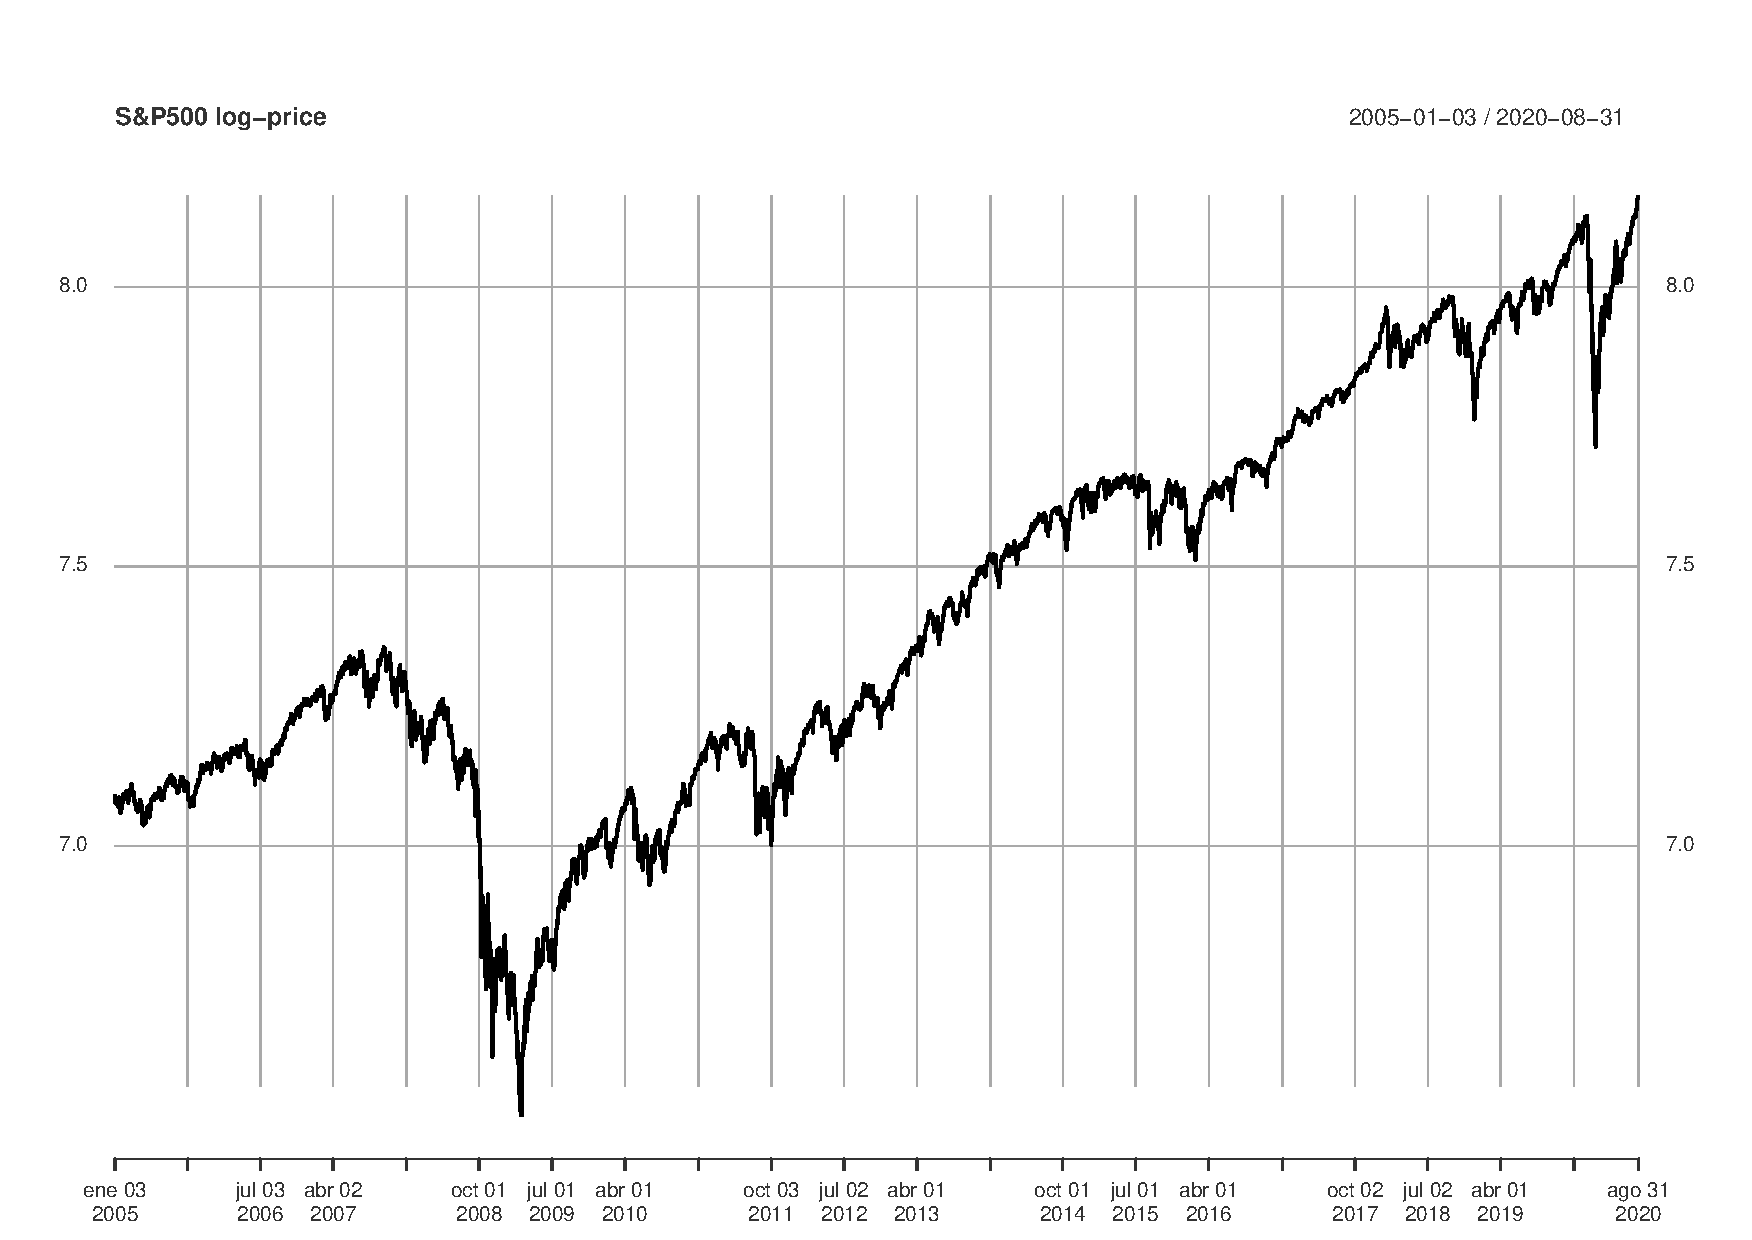
\includegraphics[scale=.25]{img/SP500}
%		\caption{S\&P 500 log-prices}
%	\end{figure}
\end{frame}

\begin{frame}{Data}
\begin{columns}
\begin{column}{.7\textwidth}
\begin{figure}
	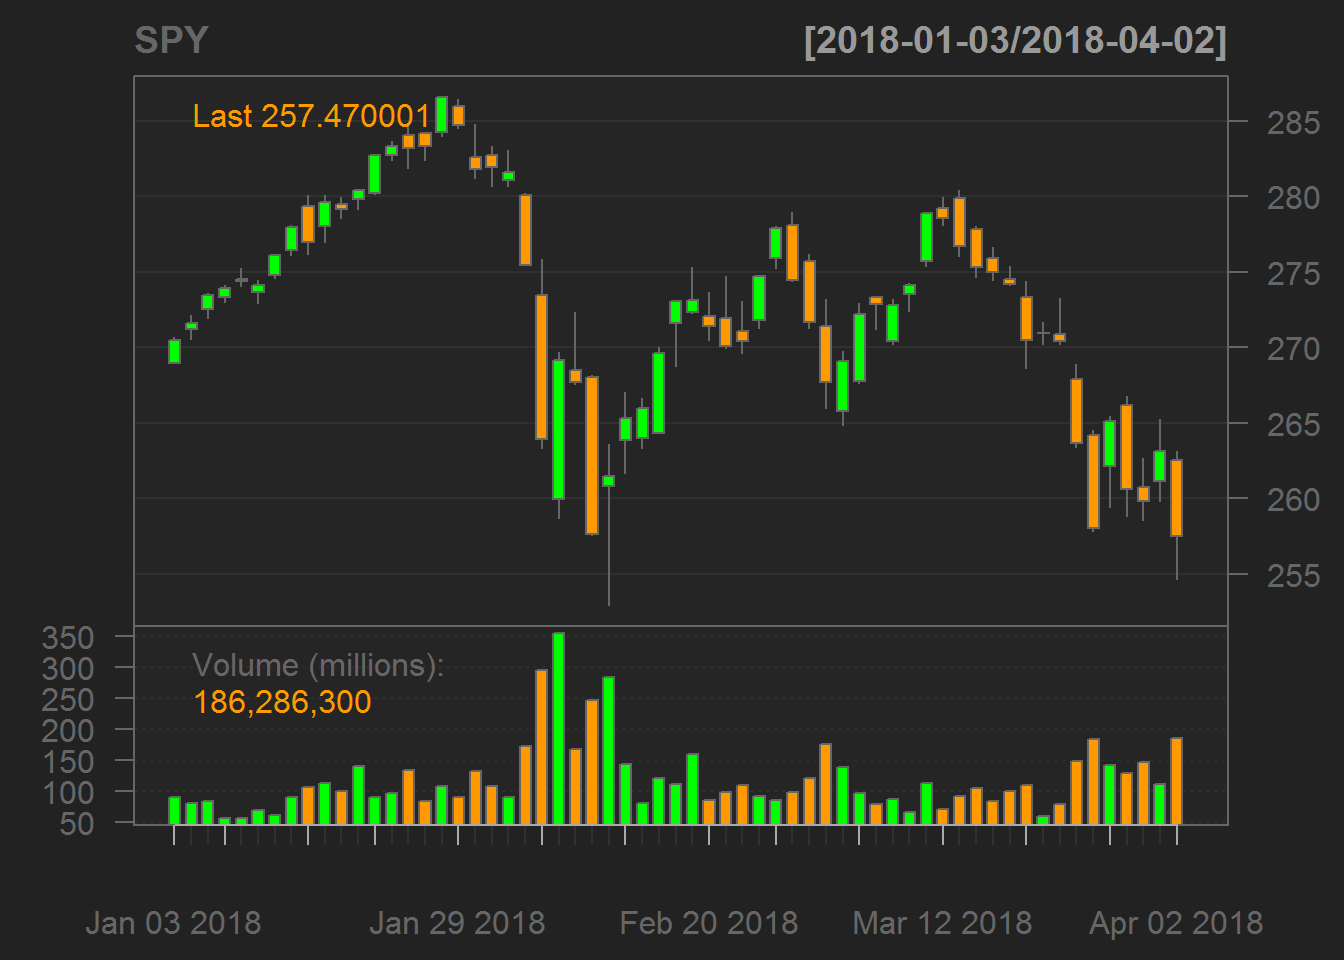
\includegraphics[width=\textwidth]{img/SPYPriceVolume}
	\caption{Price and volume chart}		
\end{figure}
\end{column}

\begin{column}{.3\textwidth}
\begin{center}
	\textbf{\underline{S\&P 500}}
\end{center}
\vspace{-.2cm}
\begin{itemize}
	\item \textbf{Meta-labeling:} 
	\newline Daily data
	
	\vspace{.15cm}
	\item \textbf{Fractional differentiation:} 
	\newline Open, High, Low, Close (OHLC)
	
	\vspace{.15cm}
	\item \textbf{Data bars:} \newline Tick data
\end{itemize}
\end{column}
\end{columns}
\end{frame}

\begin{frame}{Stationary time series}

	$y_t$ presents a \textbf{positive trend} $\Rightarrow$ Non-stationary. To 
	solve that, \textbf{log-returns} are computed: $r_t = (1-B)y_t$, where 
	$B$ is the \textbf{backshift} operator: $B y_t = y_{t-1}$.
%	
%	It is often the case that the log-prices time series $\{y_t\}$ is not 
%	stationary.\\	
%	
%	\vspace{.2cm}
%	To solve that, the time series is differentiated $r_t = (1 - B) y_t = 
%	y_t - y_{t-1}$, where $B$ is the backshift operator ($B y_t = y_{t-1}$)
	
	\begin{figure}[hbtp]
	\centering
		\includegraphics[scale=0.3]{"\homeCTwo/img/tSeriesMemory"}
		%\caption{Memory of differentiated series}\end{figure}
	\end{figure}
	
%	\vspace{-.2cm}
%	However, memory is lost in the process, begging the question: is there a 
%	trade off between stationarity and memory?

\end{frame}

\begin{frame}{Side of a position}

\begin{block}{Long position}
A long position (or going long on some stock) is the most common way to 
invest. It just means that you buy an asset and you sell it at some point, 
expecting to earn a positive return.
\end{block}

\begin{block}{Short position}
If you short a stock, you first sell a stock that someone has lent you and 
then try to repurchase it at a lower price to return the stock to the lender. 
That way, if the \textbf{stock goes down in price}, you would \textbf{earn a 
profit} by selling high and buying low.
\end{block}

%\begin{equation*}
%	R_{t_1}^{\text{short}} = \frac{\text{profits}}{p_{t_0}} = \frac{p_{t_0} - 
%	p_{t_1}}{p_{t_0}} = -R_{t_1}
%\end{equation*}

\end{frame}

\begin{frame}{Financial Metrics}

%\begin{block}{\centering{Sharpe Ratio}}
%	\begin{center}
%		$\text{SR} := \frac{\mathbb{E}[R_t - r_f]}{\sqrt{\text{Var}[R_t - 
%		r_f]}}$, representing the reward per unit of risk.
%	\end{center}
%\end{block}

%\begin{block}{\centering{Information Ratio}}
%	\begin{center}
%		$\text{IR} := \frac{\mathbb{E}[R_t - R_b]}{\sqrt{\text{Var}[R_t - 	
%		R_b]}}$, where $R_b$ are the returns of a benchmark.
%	\end{center}
%\end{block}

%\begin{block}{\centering{Drawdown}}
%	\begin{center}
%		It measures the relative drop from a historical peak.
%		\vspace{-.15cm}
%		\begin{equation*} 
%			D(t) := \frac{\text{HWM}(t) - p_t}{\text{HWM}(t)} \text{, where } 
%			\text{HWM}(t) = \max_{1 \leq \tau \leq t} p_{\tau}
%		\end{equation*}
%	\end{center}
%\end{block}

%\textbf{\underline{Sharpe Ratio:}} It represents the \textbf{reward per unit 
%of risk}.\\
%
%\begin{equation*}
%	\text{SR} := \frac{\mathbb{E}[R_t - r_f]}{\sqrt{\text{Var}[R_t - 'r_f]}}
%\end{equation*}
%
%\textbf{\underline{Drawdown:}} It measures the \textbf{relative drop} from a 
%\textbf{historical peak}.
%
%\begin{equation*} 
%	D(t) := \frac{\text{HWM}(t) - p_t}{\text{HWM}(t)} \text{, where } 
%	\text{HWM}(t) = \max_{1 \leq \tau \leq t} p_{\tau}
%\end{equation*}

\begin{columns}
\begin{column}{.5\textwidth}
\textbf{\underline{Sharpe Ratio:}} It represents the \textbf{reward per unit 
of risk}.\\

\begin{equation*}
	\text{SR} := \frac{\mathbb{E}[R_t - r_f]}{\sqrt{\text{Var}[R_t - r_f]}}
\end{equation*}
\end{column}

\begin{column}{.5\textwidth}

\textbf{\underline{Drawdown:}} It measures the \textbf{relative drop} from a 
\textbf{historical peak}.

\begin{equation*} 
	D(t) := \frac{\text{HWM}(t) - p_t}{\text{HWM}(t)}
\end{equation*}

where $\text{HWM}(t) = \max\limits_{1 \leq \tau \leq t} p_{\tau}$

\end{column}
\end{columns}

\vspace{-.5cm}
\begin{columns}
\begin{column}{.5\textwidth}
\begin{figure}
	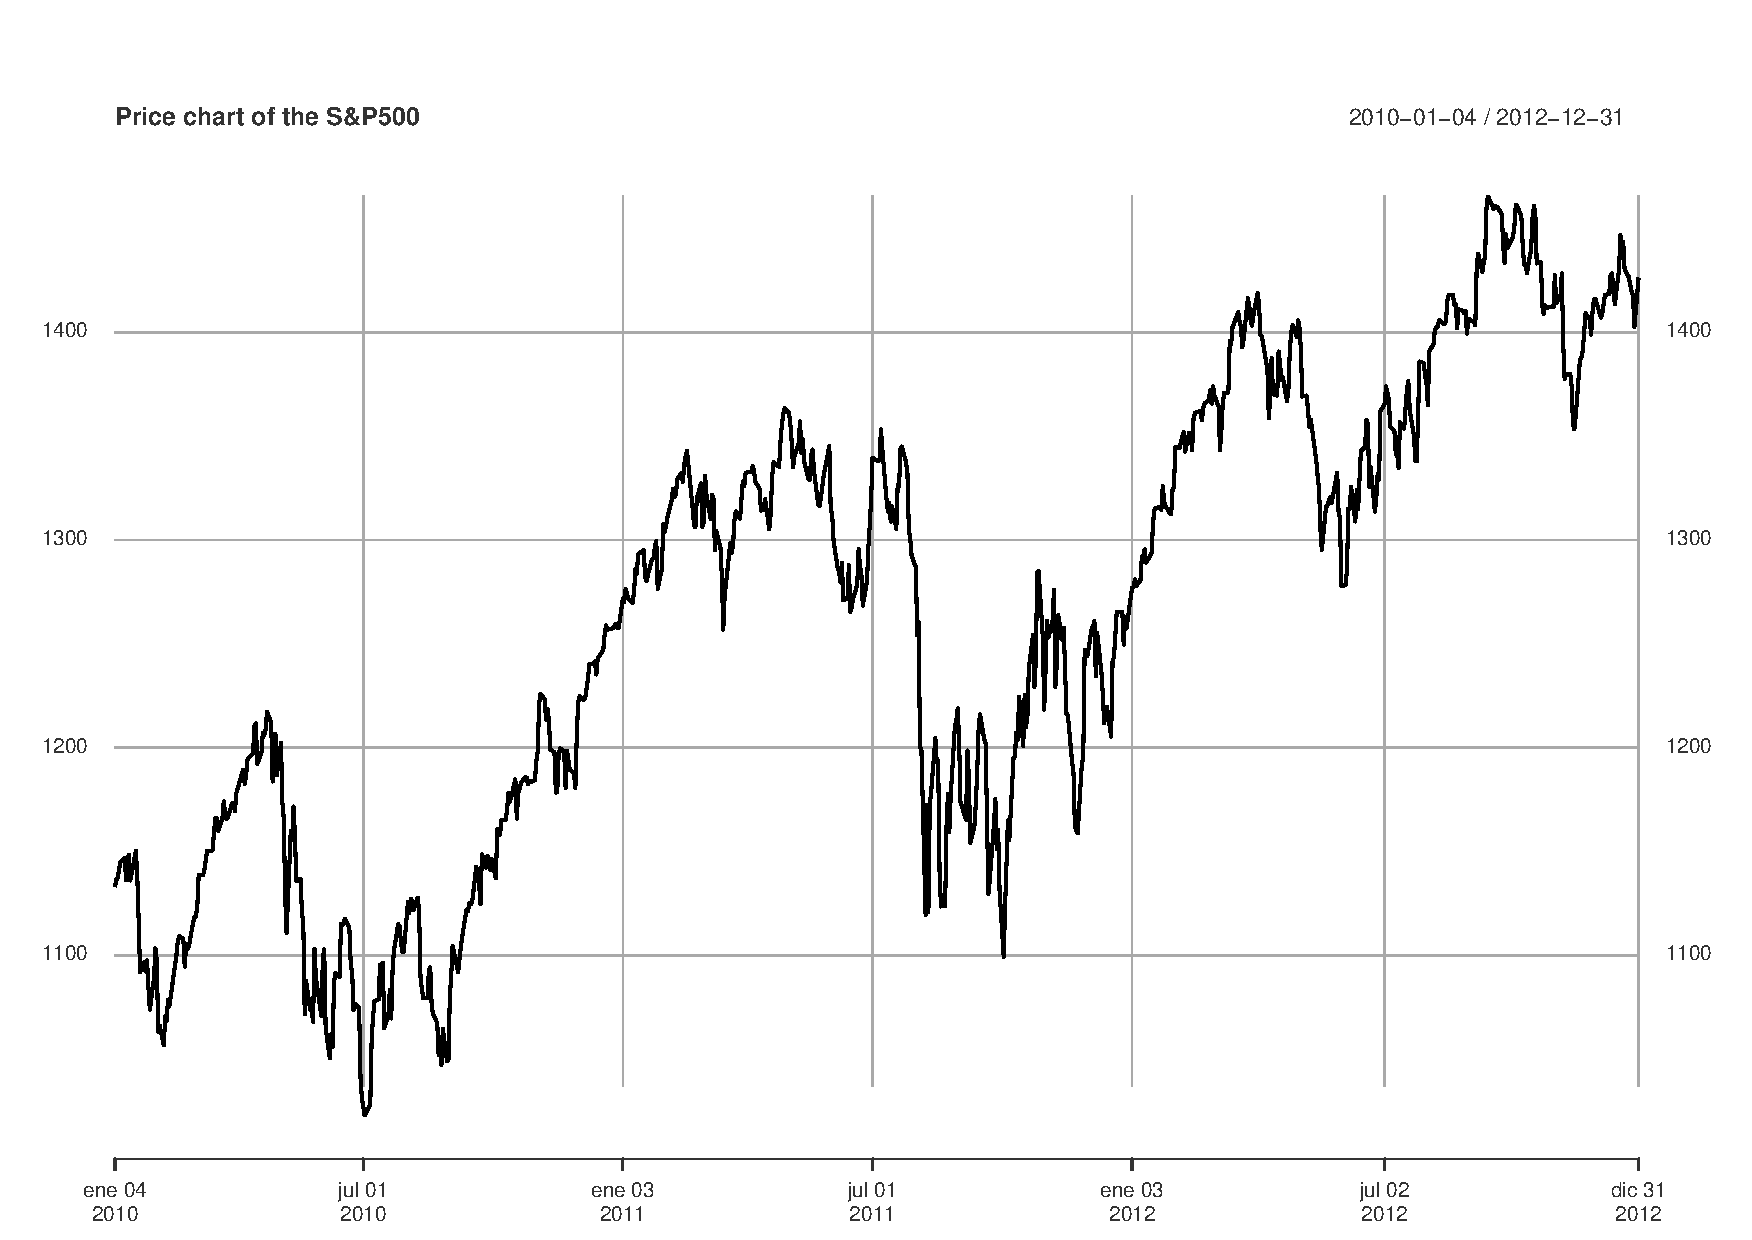
\includegraphics[scale=.2]{img/priceBasic}
\end{figure}
\end{column}

\begin{column}{.5\textwidth}
\begin{figure}
	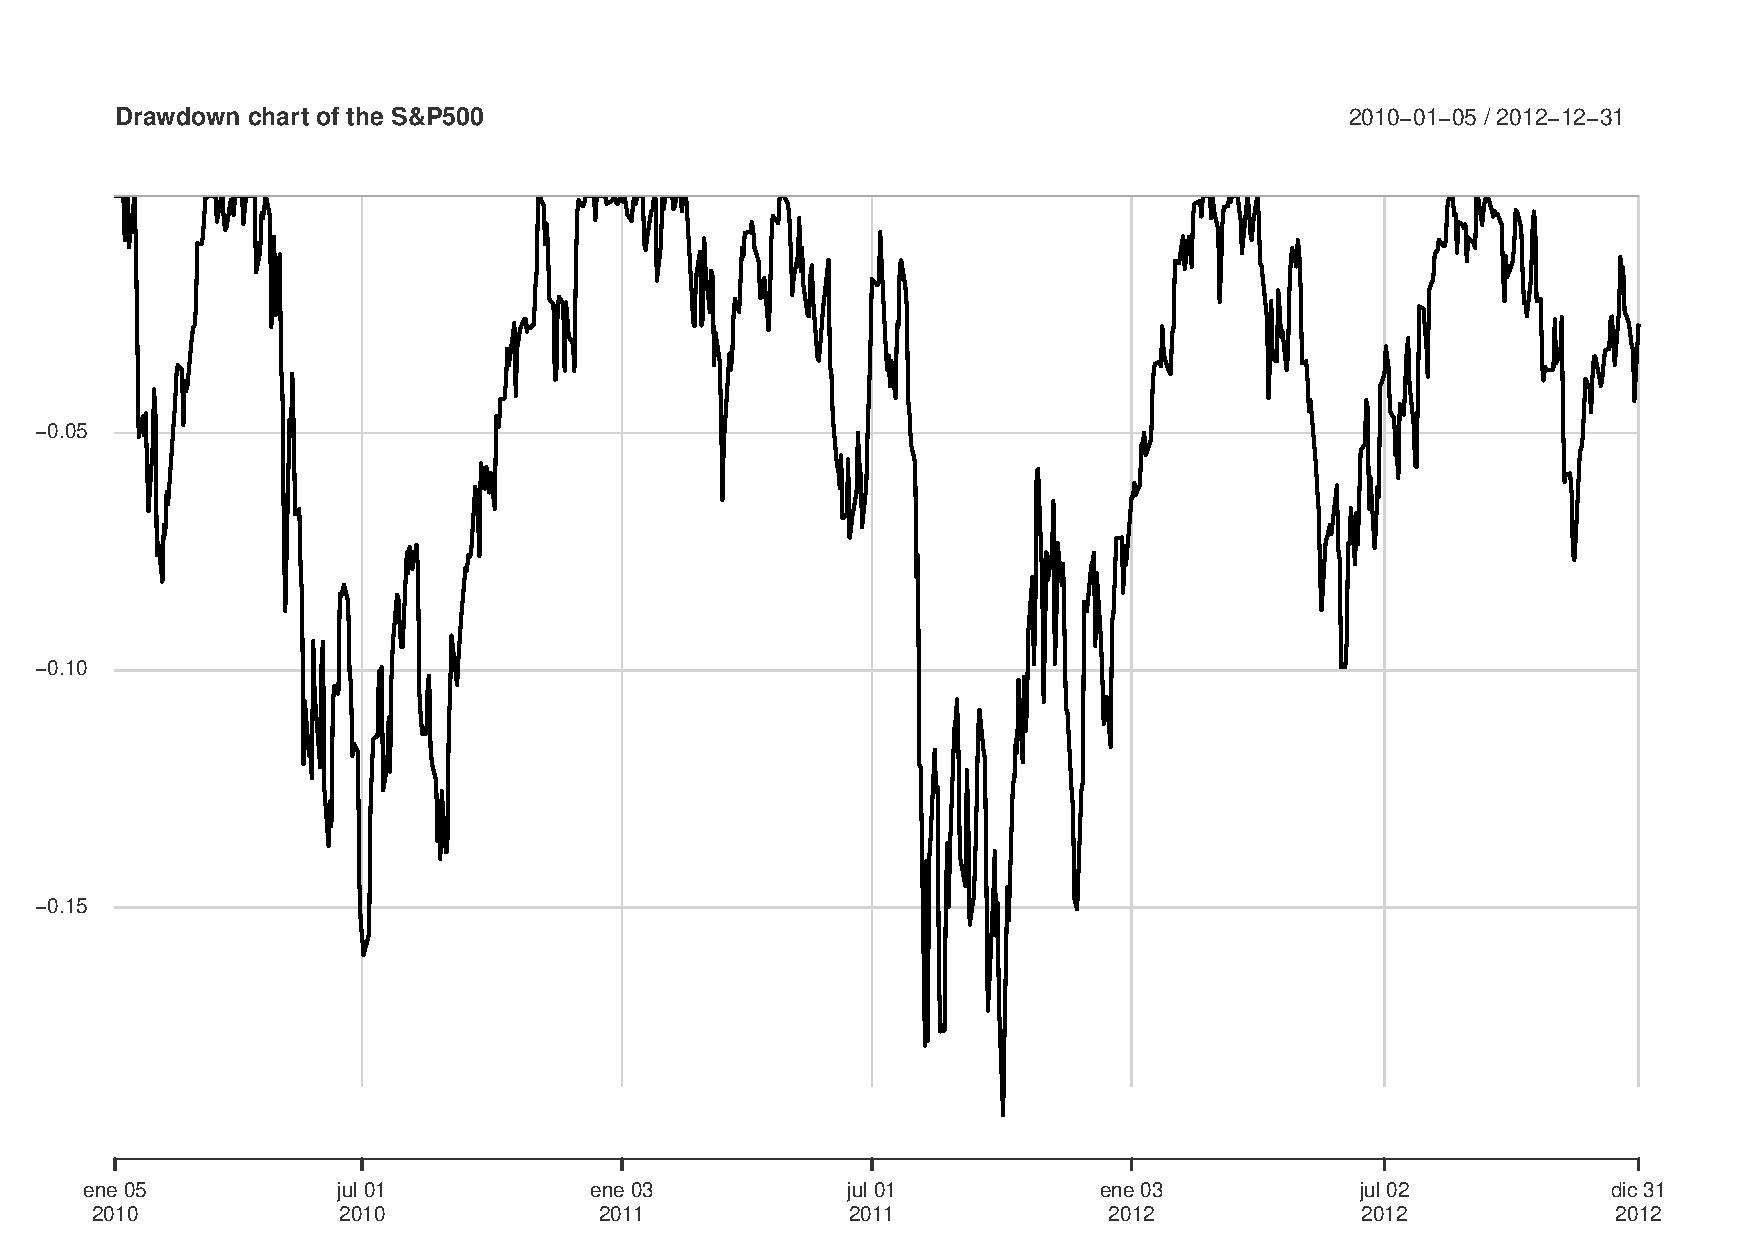
\includegraphics[scale=.2]{img/drawDownBasic}
\end{figure}
\end{column}
\end{columns}

\end{frame}


\section{Meta-labeling}
\frame{\tableofcontents[currentsection]}
%\begin{frame}{Binary classification problem}
%\begin{columns}
%\begin{column}{.5\textwidth}
%	\begin{itemize}
%		\item \textbf{Features:} $\mathbf{x} = [x_1,\ldots,x_m]$	
%		
%		\item \textbf{Target:} $y \in \{-1,+1\}$
%	\end{itemize}
%	
%	\vspace{.5cm}
%	\hspace{.25cm} \textbf{Goal:} Learn $f$ such that $y = f(\mathbf{x})$
%\end{column}
%\begin{column}{.5\textwidth}
%	\vspace{-.5cm}
%	\begin{figure}
%		\centering
%		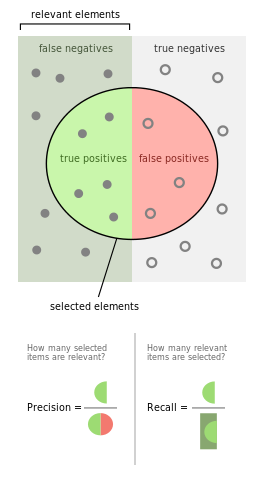
\includegraphics[scale=.45]{img/precisionRecall}	
%	\end{figure}		
%\end{column}
%\end{columns}

%\begin{itemize}
%	\centering
%	\item \textbf{Features:} $\mathbf{x} = [x_1,\ldots,x_m]$	
%	
%	\vspace{.25cm}
%	\item \textbf{Target:} $y \in \{-1,+1\}$
%\end{itemize}
%
%\begin{center}
%\vspace{.5cm}
%\hspace{.25cm} \textbf{Goal:} Estimate $f$ such that $y = f(\mathbf{x})$
%\end{center}	
%	
%\end{frame}

\begin{frame}{What is meta-labeling?}
	\begin{block}{Primary model (M1)}
		Binary classifier that will \textbf{predict} the \textbf{side of the 
		investment}. In this work, two different primary models will be 
		explored:
		
%		The 	labels will 	be noted as $y_i^{\text{M1}} \in \{-1, 1\}$ and the 
%		predictions as $\widehat{y}_i^{\text{M1}}$.\\
		
		\begin{itemize}
			\item Moving average (MA) based
			\item Machine Learning (ML) based
		\end{itemize}
	\end{block}
	\begin{block}{Secondary model (M2)}
		Binary classifier that \textbf{predicts} whether the \textbf{primary 
		model} was \textbf{right or not}. The meta-labels will be defined as:
		\scalebox{0.8}{		
		$
			y_i^{\text{M2}} = 
			\begin{cases}
				1 & \text{if } y_i^{\text{M1}} = \widehat{y}_i^{\text{M1}}\\
				0 & \text{otherwise}
			\end{cases}
		$
		}
		%, while predictions will be noted as $\widehat{y}_i^{\text{M2}}$
	\end{block}
	\begin{block}{Meta-model}
		M1 + M2. It will \textbf{only open a position}, with the side 
		predicted by M1, \textbf{when M2 determines that M1 is right}.
	\end{block}
\end{frame}


\begin{frame}{Why should meta-labeling be used?}
	\begin{itemize}
		\item Exogenous model that can work on top of a fundamental approach 
		(it avoids the ML \textbf{black box} stigma).
		
		\vspace{.25cm}
		\item Enables more \textbf{sophisticated strategies} by decoupling 
		side from size.
		
		\vspace{.25cm}
		\item \textbf{Avoids overfitting} by giving the ability to pass.
	\end{itemize}
	
\end{frame}

%\begin{frame}{Data}
%\begin{figure}[htbp]
%	\centering
%	\includegraphics[scale=.2]{"\homeCOne/img/removalOutliersGMVP"}
%	\caption{Imputed log-price time series of the S\&P 500 GMVP}
%	\label{fig:removalOutlierGMVP}
%\end{figure}
%
%\vspace{-.4cm}
%
%\begin{figure}[htbp]
%	\centering
%	\includegraphics[scale=.05]{"\homeCOne/img/dataDivision"}
%	%\caption{Data Division}
%	%\label{fig:dataDivision}
%\end{figure}
%
%\end{frame}

\begin{frame}{Labeling in financial time series}
\framesubtitle{Triple Barrier Method}

\begin{itemize}
	\item \textbf{Horizontal barriers:} Dynamic levels that depend 
	on the 10 day rolling volatility. They can be symmetric or not.
	
	\item \textbf{Vertical barrier:} Set as a fixed time horizon. 
	In this case, 10 days.
\end{itemize}

\begin{columns}
\begin{column}{.7\textwidth}
\begin{figure}[htbp]
	\centering
	\includegraphics[scale=.08]
	{"\homeCOne/img/tripleBarrierSymmetric"}
	\caption{Symmetrical horizontal barriers}
\end{figure}
\end{column}
\begin{column}{.35\textwidth}
	\textbf{Train} data set: one will be able to ``see the future'' and train 
	the algorithms accordingly.\\
	
	\vspace{.6cm}
	\textbf{Test} data set: one will try to ``predict the future'' and 
	performance will be assessed.
\end{column}
\end{columns}

\end{frame}	
% cmd + T <--> cmd + U
%\begin{frame}{Models}
%
%	\begin{block}{\centering{Moving Average (MA) based}}
%	\begin{columns}
%	\begin{column}{.5\textwidth}
%	\centering
%	\textbf{\underline{Primary model}}\\
%	
%	\begin{itemize}
%		\item Pt.1
%		
%		\item Pt.2
%	\end{itemize}
%	
%	\end{column}
%	
%	\begin{column}{.5\textwidth}
%	\centering
%	\textbf{\underline{Secondary model}}\\
%	
%	\begin{itemize}
%		\item Pt.1
%		
%		\item Pt.2
%	\end{itemize}
%	
%	\end{column}
%	\end{columns}
%
%	\end{block}
%
%	\begin{block}{\centering{Machine Learning (ML) based}}
%	\begin{columns}
%	\begin{column}{.5\textwidth}
%	\centering
%	\textbf{\underline{Primary model}}\\
%	
%	\begin{itemize}
%		\item Pt.1
%		
%		\item Pt.2
%	\end{itemize}
%	
%	\end{column}
%	
%	\begin{column}{.5\textwidth}
%	\centering
%	\textbf{\underline{Secondary model}}\\
%	
%	\begin{itemize}
%		\item Pt.1
%		
%		\item Pt.2
%	\end{itemize}
%	
%	\end{column}
%	\end{columns}
%
%	\end{block}
%\end{frame}

\begin{frame}{Results}
\framesubtitle{MA based}

	\vspace{-.1cm}
	\begin{figure}
		\centering
		\includegraphics[scale=.25]{"\homeCOne/img/Plots_MA_Test"}
	\end{figure}
	
	\vspace{-.35cm}
%	\begin{columns}
%	\begin{column}{.45\textwidth}
%		\begin{figure}
%			\centering
%			\includegraphics[scale=.2]{"\homeCOne/img/Plots_MA_Test"}
%		\end{figure}
%
%	\end{column}		
%	\begin{column}{.45\textwidth}
%		\begin{figure}
%			\centering
%			\includegraphics[scale=.2]{"\homeCOne/img/Drawdown_MA_Test"}
%		\end{figure}		
%	
%	\end{column}		
%	\end{columns}
	
	\begin{table}[htbp]
		\scriptsize
		\centering
		\caption{MA based metrics in the Test data set}
		\vspace{-.2cm}
		\begin{tabular}{ |C{2cm}|C{2.5cm}|C{2cm}| }
			\hline
			Model 			& Max. Drawdown & Sharpe Ratio\\
			\hline
			\cellcolor{Red!55} Buy \& Hold & \cellcolor{Red!55} 15.20\% &
			\cellcolor{Red!55} 0.97\\ 
			\cellcolor{ForestGreen!55} Primary model & 
			\cellcolor{ForestGreen!55} 34.41\% &
			\cellcolor{ForestGreen!55} -0.75\\ 
			\cellcolor{RoyalBlue!55} Meta-model & \cellcolor{RoyalBlue!55} 
			5.02\% &
			\cellcolor{RoyalBlue!55} 0.49\\ 
			\hline
		\end{tabular}
	\end{table}
	
%		\begin{table}[htbp]
%		\scriptsize
%		\centering
%		\caption{MA based metrics in the Test data set}
%		\vspace{-.2cm}
%		\begin{tabular}{ |C{2cm}|C{2.5cm}|C{2cm}| }
%			\hline
%			Model 			& Max. Drawdown & Sharpe Ratio\\
%			\hline
%			Buy \& Hold 		& \cellcolor{Goldenrod!45} 15.20\% &
%			\cellcolor{SpringGreen!45} 0.97\\ 
%			Primary model 	& \cellcolor{red!25} 34.41\% &
%			\cellcolor{red!25} -0.75\\ 
%			Meta-model 		& \cellcolor{SpringGreen!45} 5.02\% &
%			\cellcolor{Goldenrod!45} 0.49\\ 
%			\hline
%		\end{tabular}
%	\end{table}

\end{frame}

\begin{frame}{Results}
\framesubtitle{ML based}

	\vspace{-.1cm}
	\begin{figure}
		\centering
		\includegraphics[scale=.25]{"\homeCOne/img/Plots_ML_Test"}
	\end{figure}	

	\vspace{-.35cm}	
%	\begin{columns}
%	\begin{column}{.45\textwidth}
%		\begin{figure}
%			\centering
%			\includegraphics[scale=.2]{"\homeCOne/img/Plots_ML_Test"}
%		\end{figure}
%
%	\end{column}		
%	\begin{column}{.45\textwidth}
%		\begin{figure}
%			\centering
%			\includegraphics[scale=.2]{"\homeCOne/img/Drawdown_ML_Test"}
%		\end{figure}		
%	
%	\end{column}		
%	\end{columns}
	
%	\begin{table}[htbp]
%		\scriptsize
%		\centering
%		\caption{ML based metrics in the Test data set}
%		\vspace{-.2cm}
%		\begin{tabular}{ |C{2cm}|C{2.5cm}|C{2cm}| }
%			\hline
%			Model 			& Max. Drawdown & Sharpe Ratio\\
%			\hline
%			Buy \& Hold 		& \cellcolor{SpringGreen!45} 15.20\% &
%			\cellcolor{SpringGreen!45} 0.97\\ 
%			Primary model 	& \cellcolor{red!25} 16.42\% &
%			\cellcolor{red!25} 0.66\\ 
%			Meta-model 		& \cellcolor{red!25} 16.42\% &
%			\cellcolor{red!25} 0.66\\ 
%			\hline
%		\end{tabular}
%	\end{table}

	\begin{table}[htbp]
		\scriptsize
		\centering
		\caption{ML based metrics in the Test data set}
		\vspace{-.2cm}
		\begin{tabular}{ |C{2cm}|C{2.5cm}|C{2cm}| }
			\hline
			Model 			& Max. Drawdown & Sharpe Ratio\\
			\hline
			\cellcolor{Red!55} Buy \& Hold & \cellcolor{Red!55} 15.20\% &
			\cellcolor{Red!55} 0.97\\ 
			\cellcolor{ForestGreen!55} Primary model & 
			\cellcolor{ForestGreen!55} 16.42\% &
			\cellcolor{ForestGreen!55} 0.66\\ 
			\cellcolor{RoyalBlue!55} Meta-model & \cellcolor{RoyalBlue!55} 
			16.42\% &
			\cellcolor{RoyalBlue!55} 0.66\\ 
			\hline
		\end{tabular}
	\end{table}
	
\end{frame}

\begin{frame}{Coin flip correction}
\vfill
In an attempt to create \textbf{better (but artificial) primary models}, they 
will use a \textbf{new feature} $F$:

\vfill
\begin{equation*}
	F_i = (1 - 2 \cdot S_i) \cdot y_i^{\text{M1}}
\end{equation*}

\vfill
Where:
\begin{itemize}
	\item $S_i \sim Be(p)$ is the r.v. in charge of swapping the label 
	$y_i^{\text{M1}}$
	
	\vspace{.15cm}
	\item $p = \text{Pr}(S_i = 1)$
	
	\vspace{.15cm}
	\item $y_i^{\text{M1}} \in \{-1,+1\}$ is the \textbf{label} representing 
	the \textbf{side}.
\end{itemize}
\vfill

\end{frame}

\begin{frame}{Coin flip correction}
\framesubtitle{Results}
\begin{figure}
	\centering
    \includegraphics[scale=.35]
    {"\homeCOne/img/coinFlip/coinFlipModelsSrTest"} 
    \caption{Sharpe Ratio of coin flip models (Test)}
\end{figure}

\end{frame}

\section{Fractional differentiation}
\frame{\tableofcontents[currentsection]}

\begin{frame}{Fractional differentiation}
\textbf{Stationarity} of $y_t \Rightarrow$ \textbf{Log-returns} $r_t = 
(1-B)y_t = y_t - B y_t = y_t - y_{t-1}$

\vspace{.25cm}
Is part of the \textbf{signal} lost?

%Consider the \textbf{backshift operator}, $B$, applied to a time series: 
%$B^k y_t = y_{t-k}$
%
%\vspace{.25cm}
%In order to achieve \textbf{stationarity}, the \textbf{log-returns} can be 
%calculated as: $r_t = (1-B)y_t = y_t - y_{t-1}$. However, \textbf{memory is 
%lost} in the process.

\vspace{.25cm}
\textbf{Fractionally differentiated time series:} $x_t^d = (1-B)^d \ y_t$, 
where $d \in (0,1)$ and
\begin{align*}
	(1 - B)^d = \sum_{k = 0}^{\infty} \binom{d}{k} (-B)^k
	= \sum_{k = 0}^{\infty} B^k \underbrace{(-1)^k \prod_{i = 0}^{k - 1} 
	\frac{d - i}{k - i}}_{=: w_k}
\end{align*}

\vspace{-.4cm}
\begin{align*}
	\textbf{FFD method: } (1 - B)^d = \sum_{k = 0}^{\infty} w_k B^k \approx 
	\sum_{k=0}^{l^*} w_k B^k = \phi_d(B)
\end{align*}

\vspace{-.4cm}
\begin{align*}
	x_t^d = \phi_d(B) y_t
\end{align*}	

\end{frame}

%\begin{frame}{FFD method}
%\framesubtitle{Fixed-width window fracdiff}
%\begin{columns}
%\begin{column}{.35\textwidth}
%	$w_k = w_{k-1} \cdot \frac{k-1-d}{k}$
%	
%	\vspace{-.3cm}
%	$$(1-B)^d = \sum_{k=0}^\infty w_k B^k$$
%
%	Find $l^*$ such that $|w_{l^*}| > \tau$ and $|w_{l^*+1}| \leq \tau$	
%	
%	$$\Rightarrow \sum_{k=0}^{l^*} w_k B^k =: \phi_d(B)$$
%	
%	$$x_t^d = \phi_d(B) y_t$$
%\end{column}		
%\begin{column}{.65\textwidth}
%	\begin{figure}
%		\centering
%		\includegraphics[width=.95\textwidth]{"\homeCTwo/img/weightsD"}
%		\caption{Weights, $w_k$, as a function of $d$}
%	\end{figure}		
%
%\end{column}		
%\end{columns}
%
%\end{frame}

\begin{frame}{FFD method}
	\begin{figure}
		\centering
		\includegraphics[scale=0.325]{"\homeCTwo/img/FFD"}
		\caption{Memory of differentiated time series $\left( \tau = 10^{-4}
		\right)$}
	\end{figure}
\end{frame}

\begin{frame}{FFD method}
	\begin{figure}
		\centering
		\includegraphics[scale=0.325]{"\homeCTwo/img/ADFFFD"}
		\caption{Stationary test statistic as a function of $d$}
	\end{figure}
\end{frame}


\begin{frame}{Models}
\textbf{Goal:} Determine if \textbf{fractionally differentiated} features can 
give \textbf{better} 1-day \textbf{forecasts}.

\begin{columns}
\begin{column}{.45\textwidth}
\begin{itemize}
	\item \textbf{Naive} model (benchmark): 
	\vspace{.05cm} 
	\newline $\widehat{y}_{t+1}^{\text{Close}} = y_t^{\text{Close}}$
	
	\vspace{.25cm}
	\item \textbf{FFD} model: Use the FFD method with $d^*$, the minimum 
	$d$ such that it passes the ADF test.
	
	\vspace{.25cm}
	\item \textbf{Returns} model: Use fully differentiated features 
	($d = 1$) $\Rightarrow$ log-returns.
\end{itemize}
\end{column}

\begin{column}{.45\textwidth}
	\textbf{Features:} $y_t^{\text{Open}}$, $y_t^{\text{High}}$, 
	$y_t^{\text{Low}}$ and $y_t^{\text{Close}}$

	\vspace{.25cm}
	\textbf{Target:} $y_{t+1}^{\text{Close}}$
	\vfill
\end{column}
\end{columns}

\end{frame}

\begin{frame}{Metrics}
	\vfill	
	Let's suppose that the time series $y_t$ has $T$ observations and the 
	Test data set starts at $t = n_0$. Then, one can define the following:
	
	\vfill
	\begin{itemize}
		\item \textbf{Errors:} $e_k := y_k - \widehat{y}_k$, where $k \in 
		\{n_0, \ldots, T\}$
		
		\item \textbf{Median of errors:} 
		$\widetilde{e} := \text{median}(e_k)$
	\end{itemize}
	
	\vfill
	\begin{columns}
	\begin{column}{.3\textwidth}
	\begin{block}{\centering RMSE}
		\centering
		\scalebox{0.99}{
		$\text{RMSE} = \sqrt{\frac{\sum\limits_{k=n_0}^T (e_k)^2}{T-n_0+1}}$
		}
	\end{block}
	\end{column}
	
	\begin{column}{.3\textwidth}
	\begin{block}{\centering MAPE}
	\vspace{.12cm}
		\centering
		\scalebox{0.75}{
		$
		\text{MAPE} =
		\frac{1}{T-n_0+1} \cdot \sum\limits_{k=n_0}^T \left| \frac{e_k}{y_k} 
		\right|
		$
		}
	\vspace{.12cm}
	\end{block}
	\end{column}
	
	\begin{column}{.3\textwidth}
	\begin{block}{\centering MAD}
	\vspace{.43cm}
		\centering
		\scalebox{0.75}{
		$\text{MAD} = \text{median}(e_k - \widetilde{e})$
		}
	\vspace{.43cm}	
	\end{block}				
	\end{column}
	\end{columns}
\end{frame}

\begin{frame}{Results}

\vspace{-.2cm}
\begin{figure}[htbp]
	\hspace{1.38cm}
	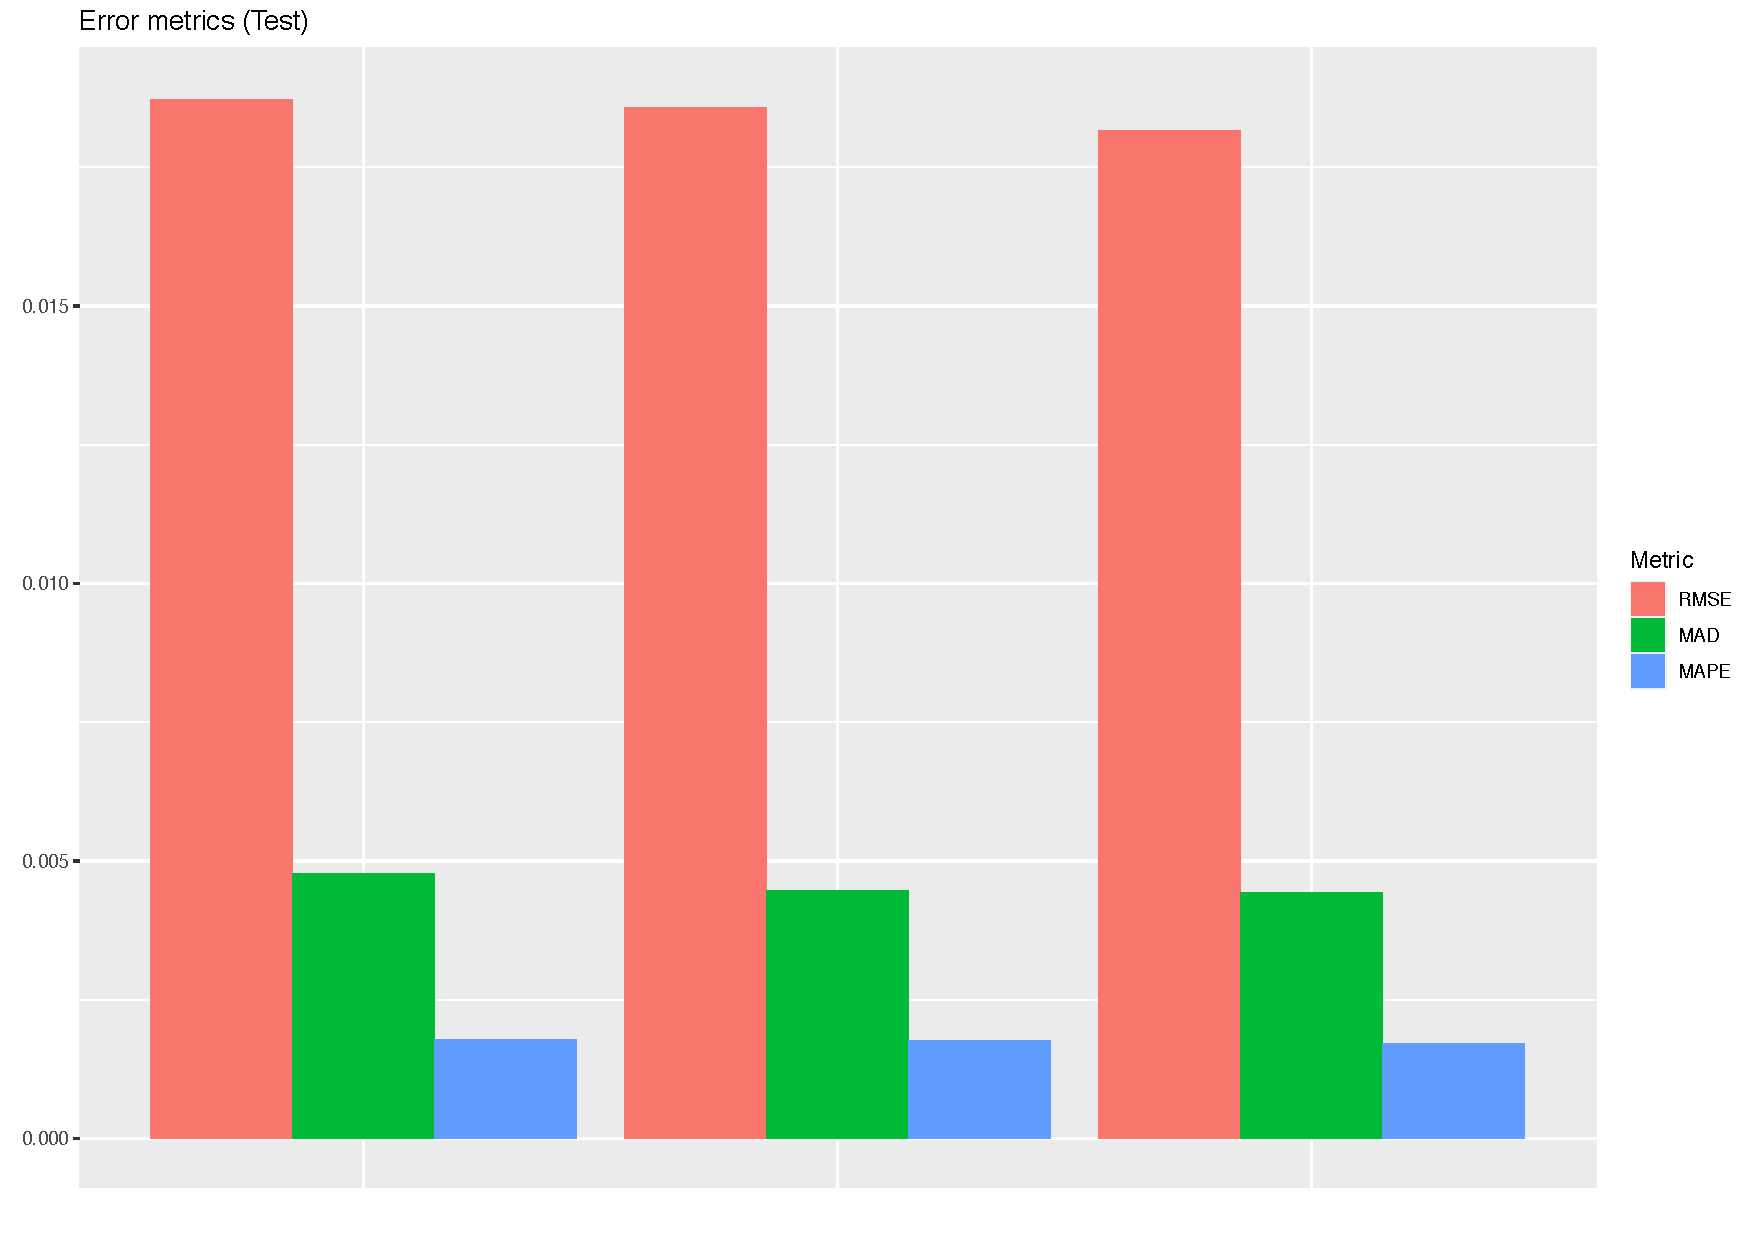
\includegraphics[scale=0.32]{img/errorMetricsFFDNoLegend}
%	\includegraphics[scale=0.32]{"\homeCTwo/img/errorMetricsFFD"}
	%\caption{Error metrics in the Test data set}
\end{figure}

\vspace{-1.02cm}
\begin{columns}
\begin{column}{.001\textwidth}
\end{column}
\begin{column}{.8\textwidth}
\begin{table}
	\centering
%	\caption{Error metrics of the models considered in the Test data set}
	\scalebox{0.7}{
	\begin{tabular}{ |C{2.9cm}|C{3.47cm}|C{3.47cm}|C{3.48cm}| }
		\hline
			 & FFD model 	& Naive model 	& Returns model\\
		\hline
		RMSE $(\times 10^{-2})$ & 1.87 (-0.78\%) & 1.86 & 1.82 (2.27\%)\\
		MAPE $(\times 10^{-3})$ & 1.79 (-1.91\%) & 1.76 & 1.72 (2.24\%)\\
		MAD \hspace{.065cm} $(\times 10^{-3})$ & 4.78 (-6.85\%) & 4.47 & 
		4.44 (0.73\%)\\
		\hline
	\end{tabular}
	}
\end{table}
\end{column}

\begin{column}{.199\textwidth}

\end{column}
\end{columns}


\end{frame}

\section{Data parsing as bars}
\frame{\tableofcontents[currentsection]}

\begin{frame}{Data bars}
\begin{columns}
\begin{column}{.3\textwidth}

\begin{center} 
	\underline{\textbf{Data:}}
\end{center}
\vspace{-.15cm}
Tick data of IVE (S\&P 500 ETF) from 2013

\begin{center} 
	\underline{\textbf{Types of bars:}} 
\end{center}
\vspace{-.15cm}
\begin{itemize}
	\item Time
	\item Volume
	\item Dollar volume
	\item Tick
\end{itemize}

\end{column}
\begin{column}{.7\textwidth}
	\begin{figure}
		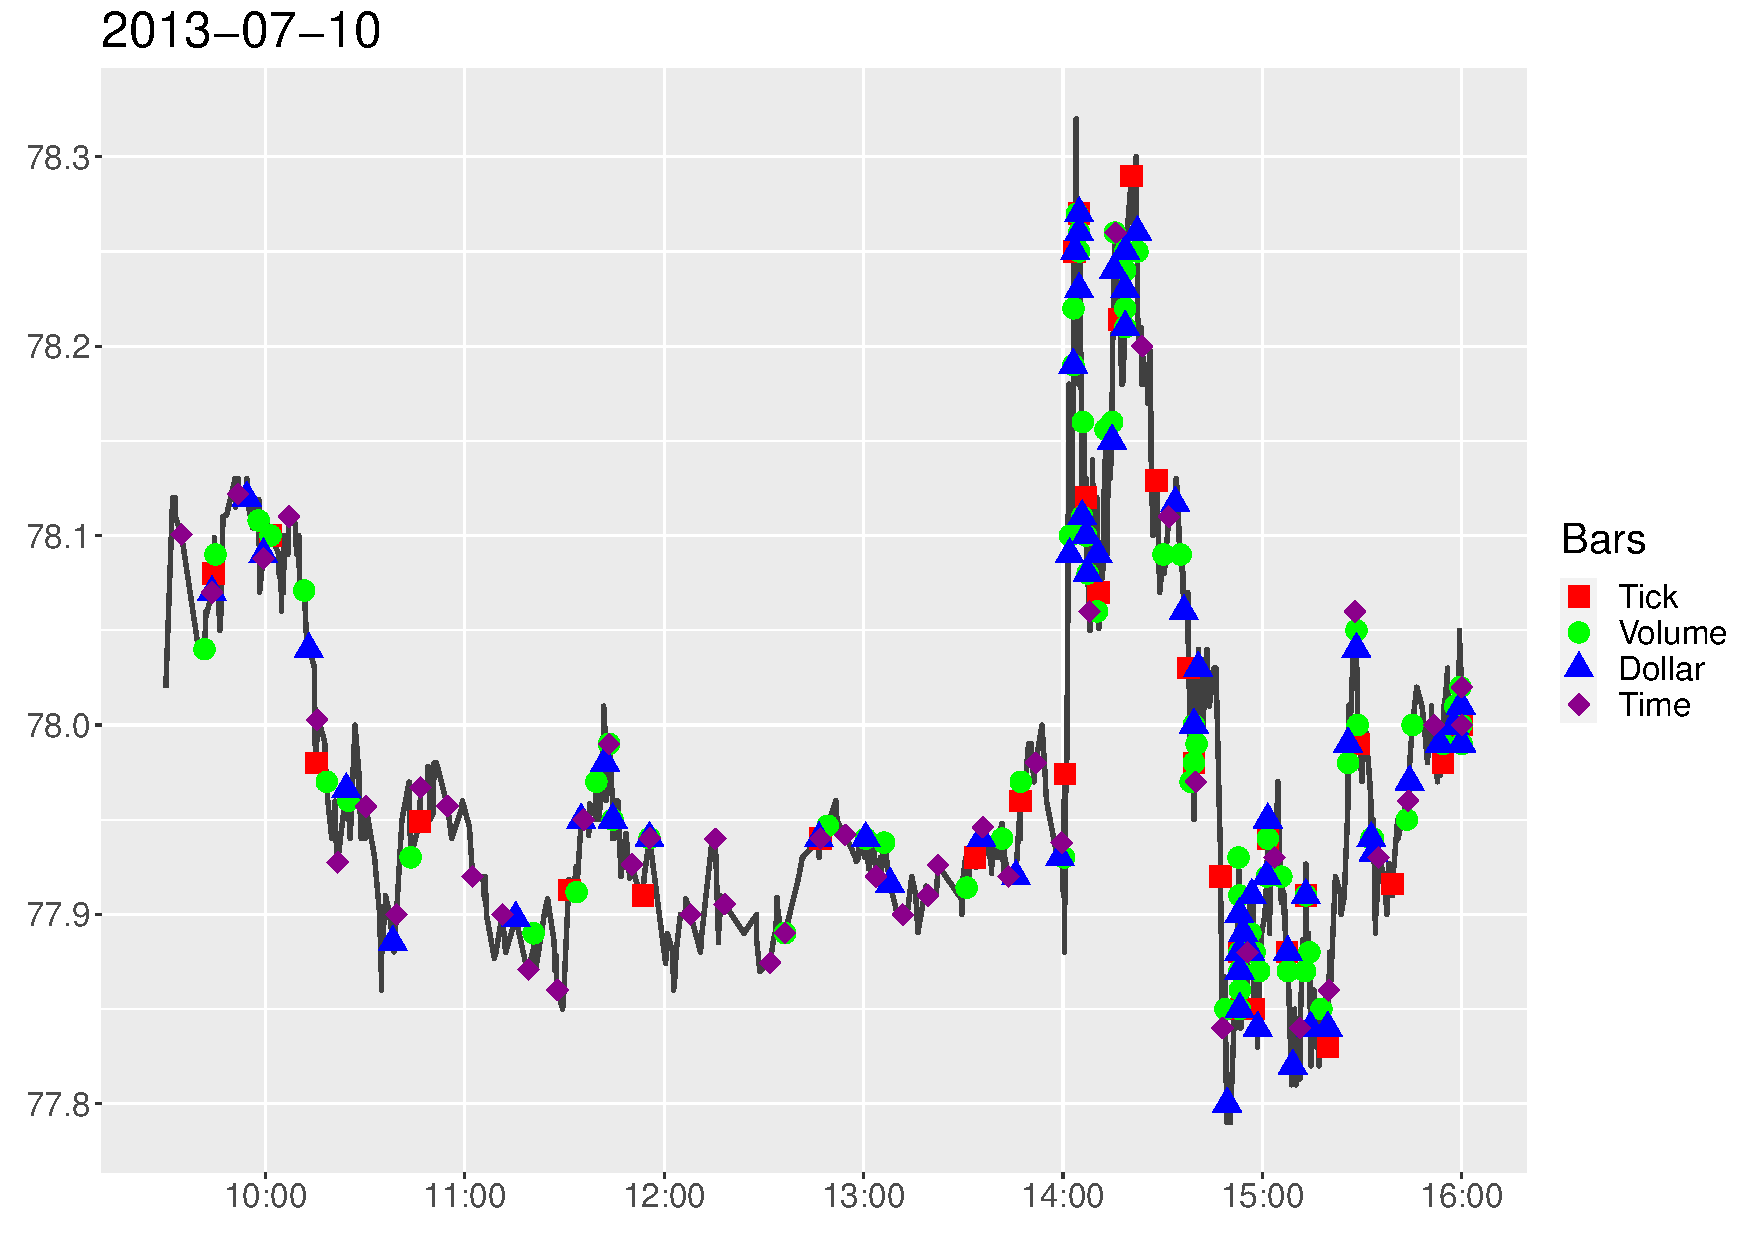
\includegraphics[width=\textwidth]{img/sampling}
	\end{figure}
\end{column}
\end{columns}
\end{frame}

\begin{frame}{Sampling}
\framesubtitle{Example day}
\begin{figure}
	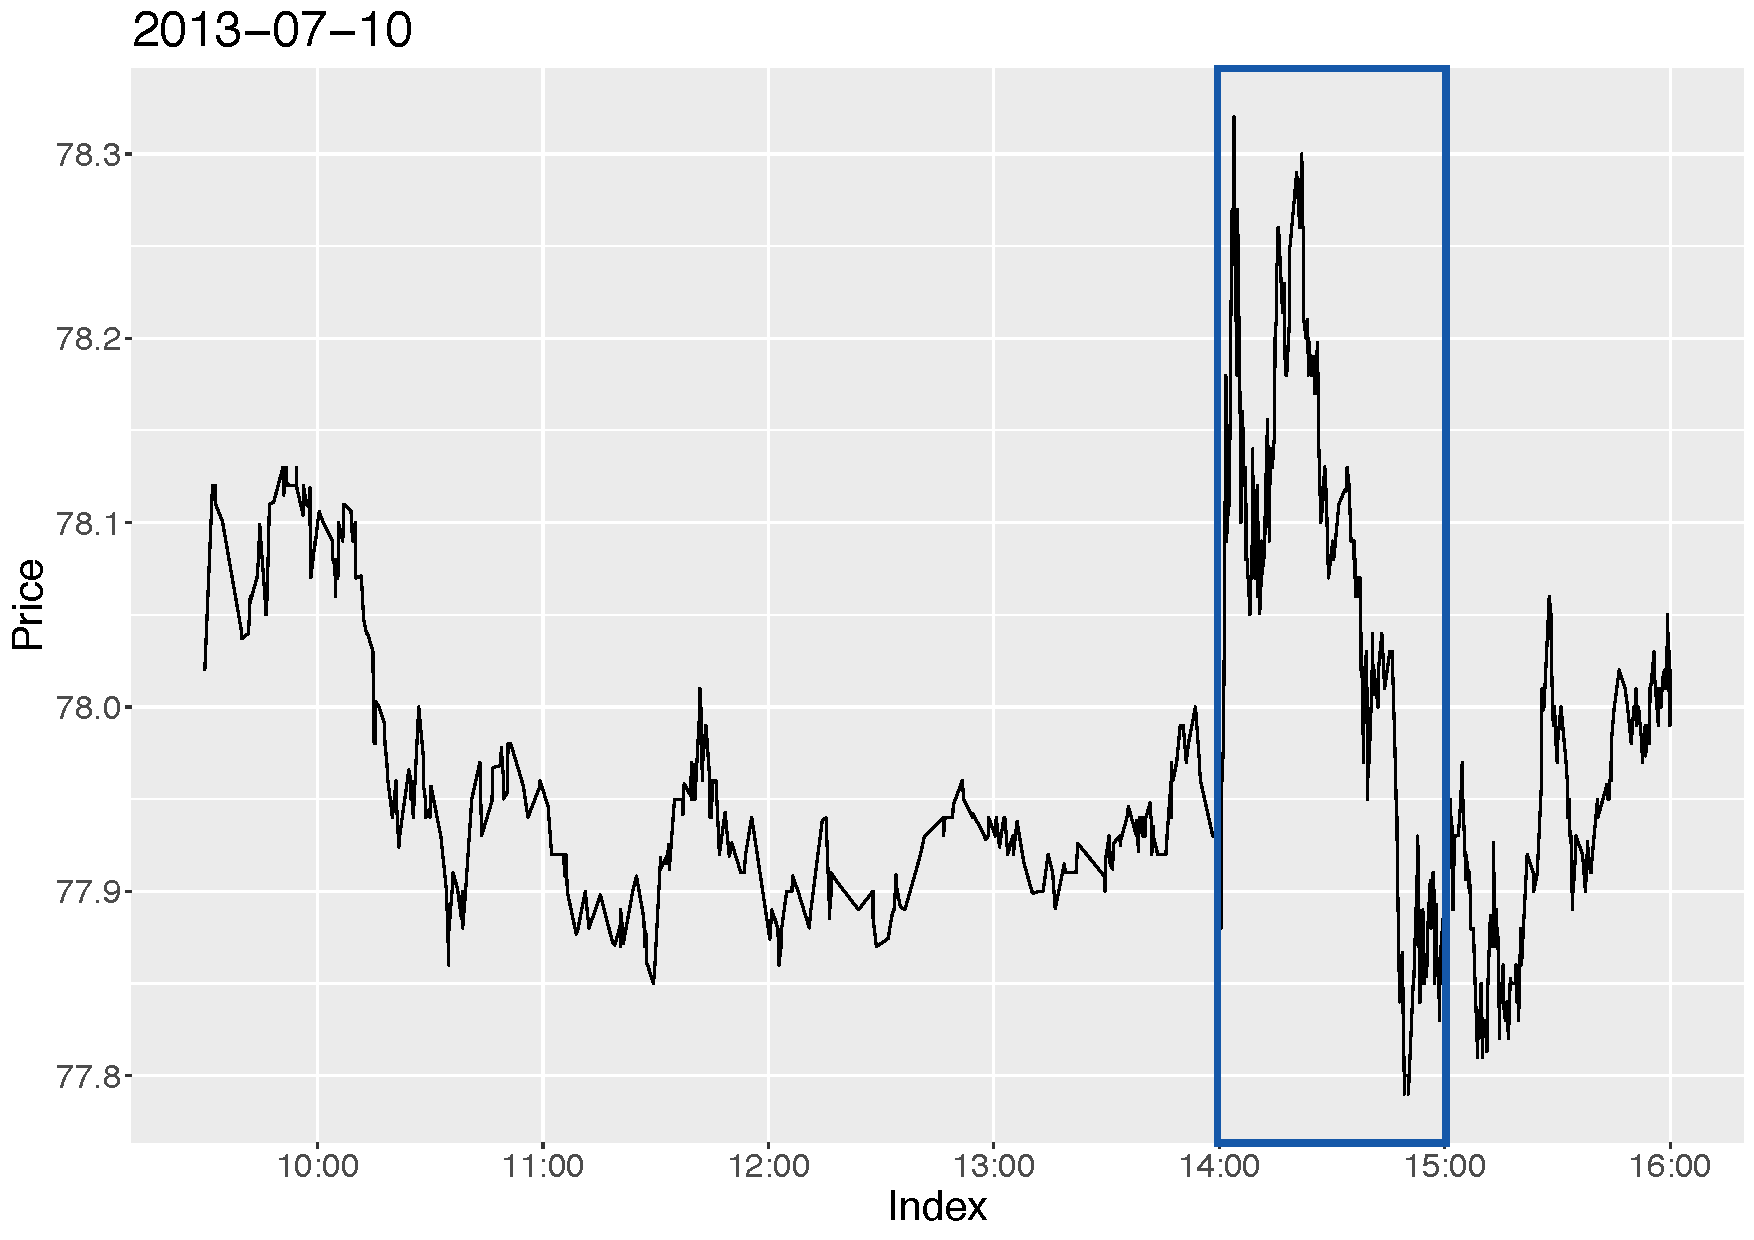
\includegraphics[scale=.35]{img/regularZoomBis}
\end{figure}
\end{frame}

\begin{frame}{Sampling}
\begin{figure}[htbp]
	\centering	
	\begin{subfigure}{.5\textwidth}
		\centering
		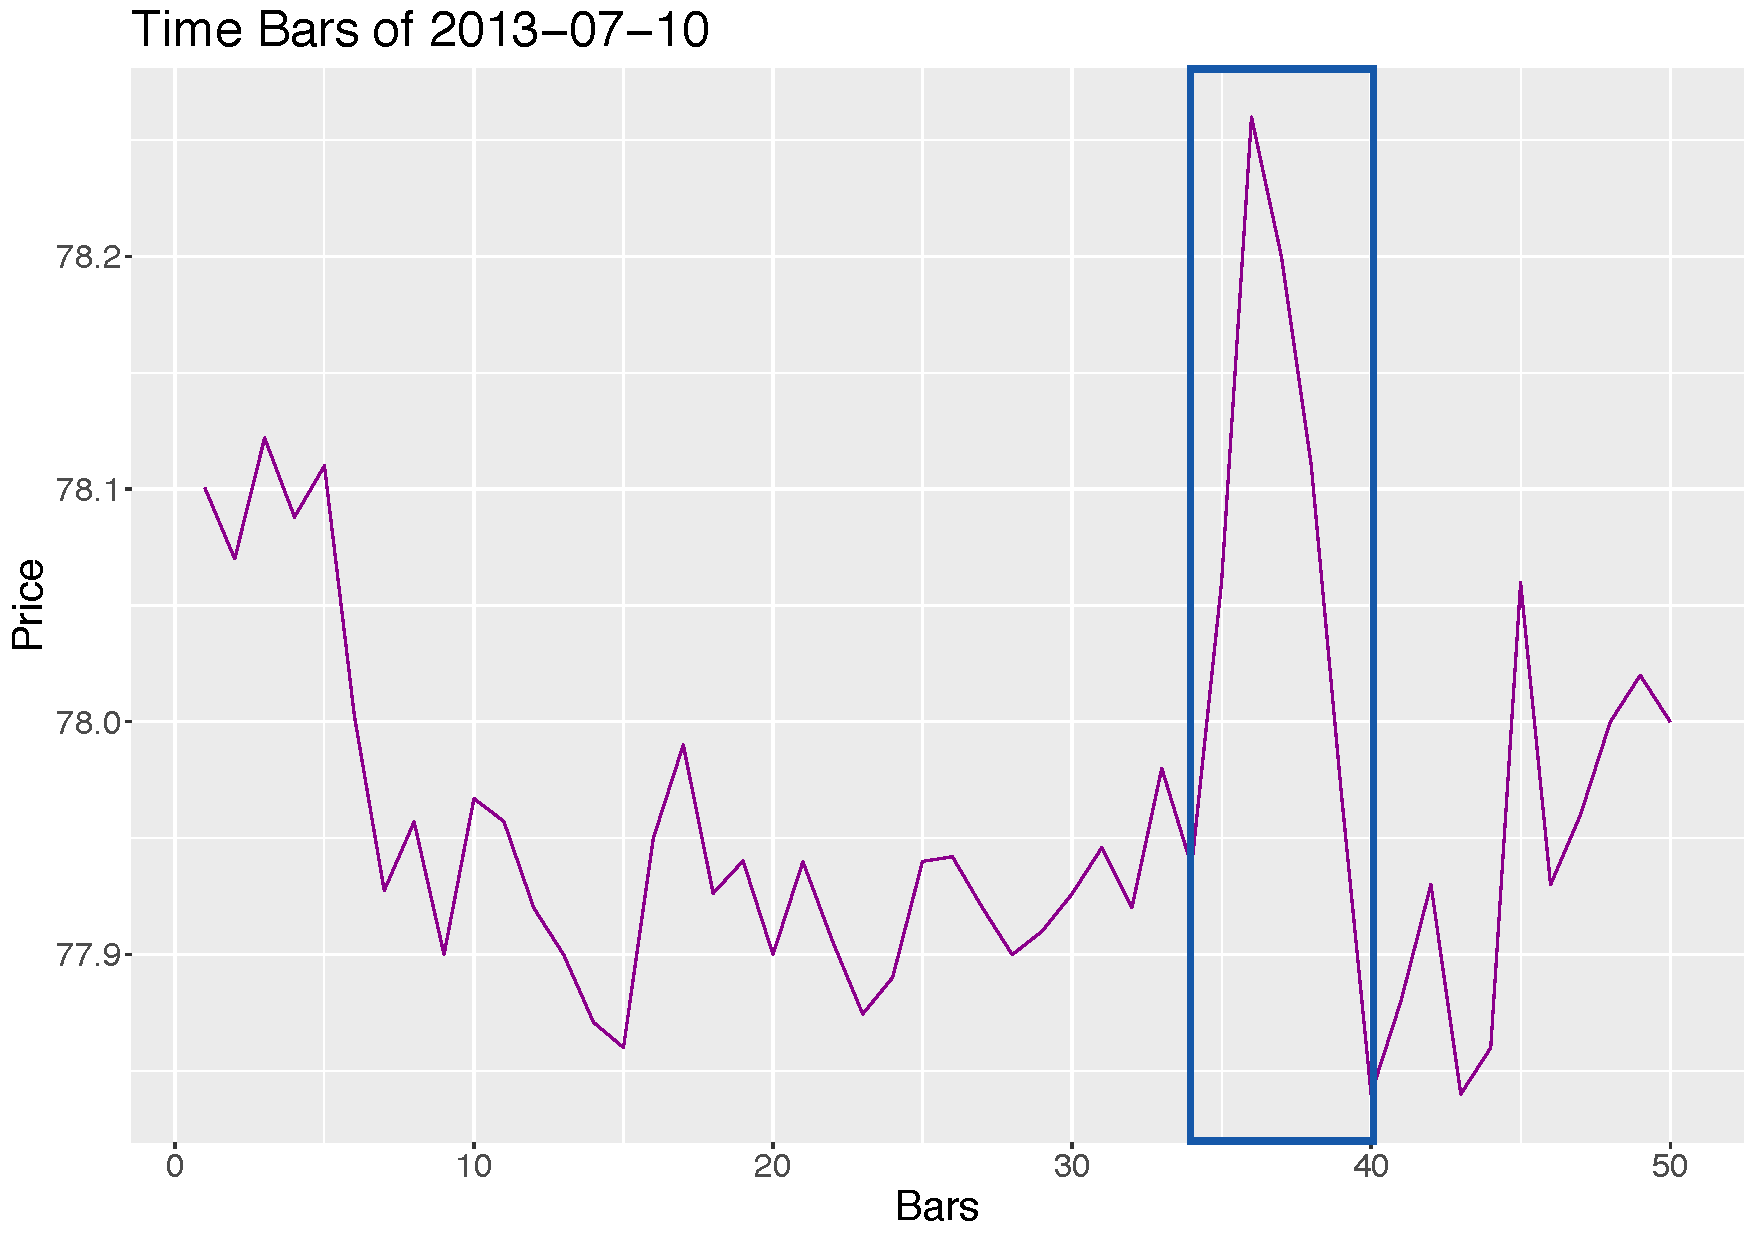
\includegraphics[scale=.15]{img/timeZoomBis}
		\caption{Time bars}
	\end{subfigure}%
	\begin{subfigure}{.5\textwidth}
		\centering
		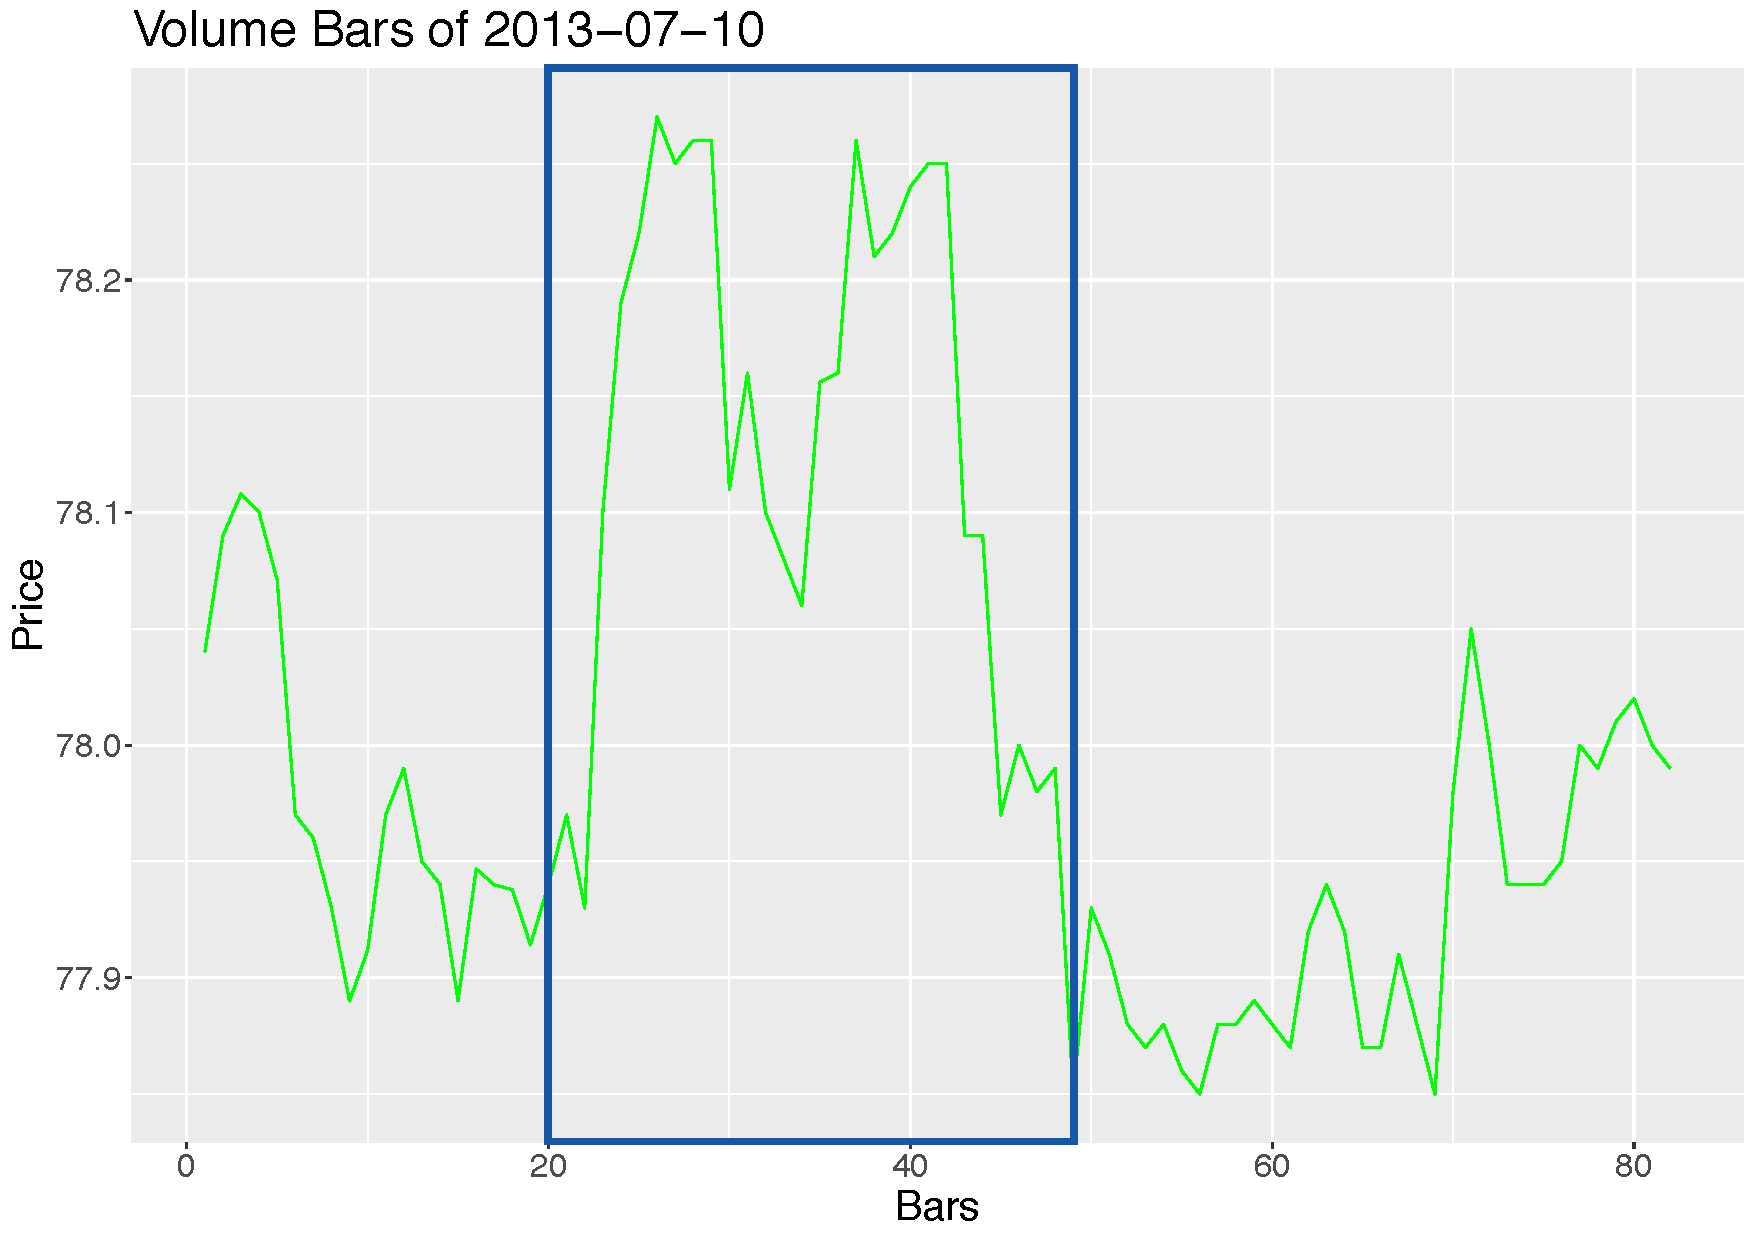
\includegraphics[scale=.15]{img/volumeZoomBis}
		\caption{Volume bars}
	\end{subfigure}%

	\vspace{.2cm}

	\begin{subfigure}{.5\textwidth}
		\centering
		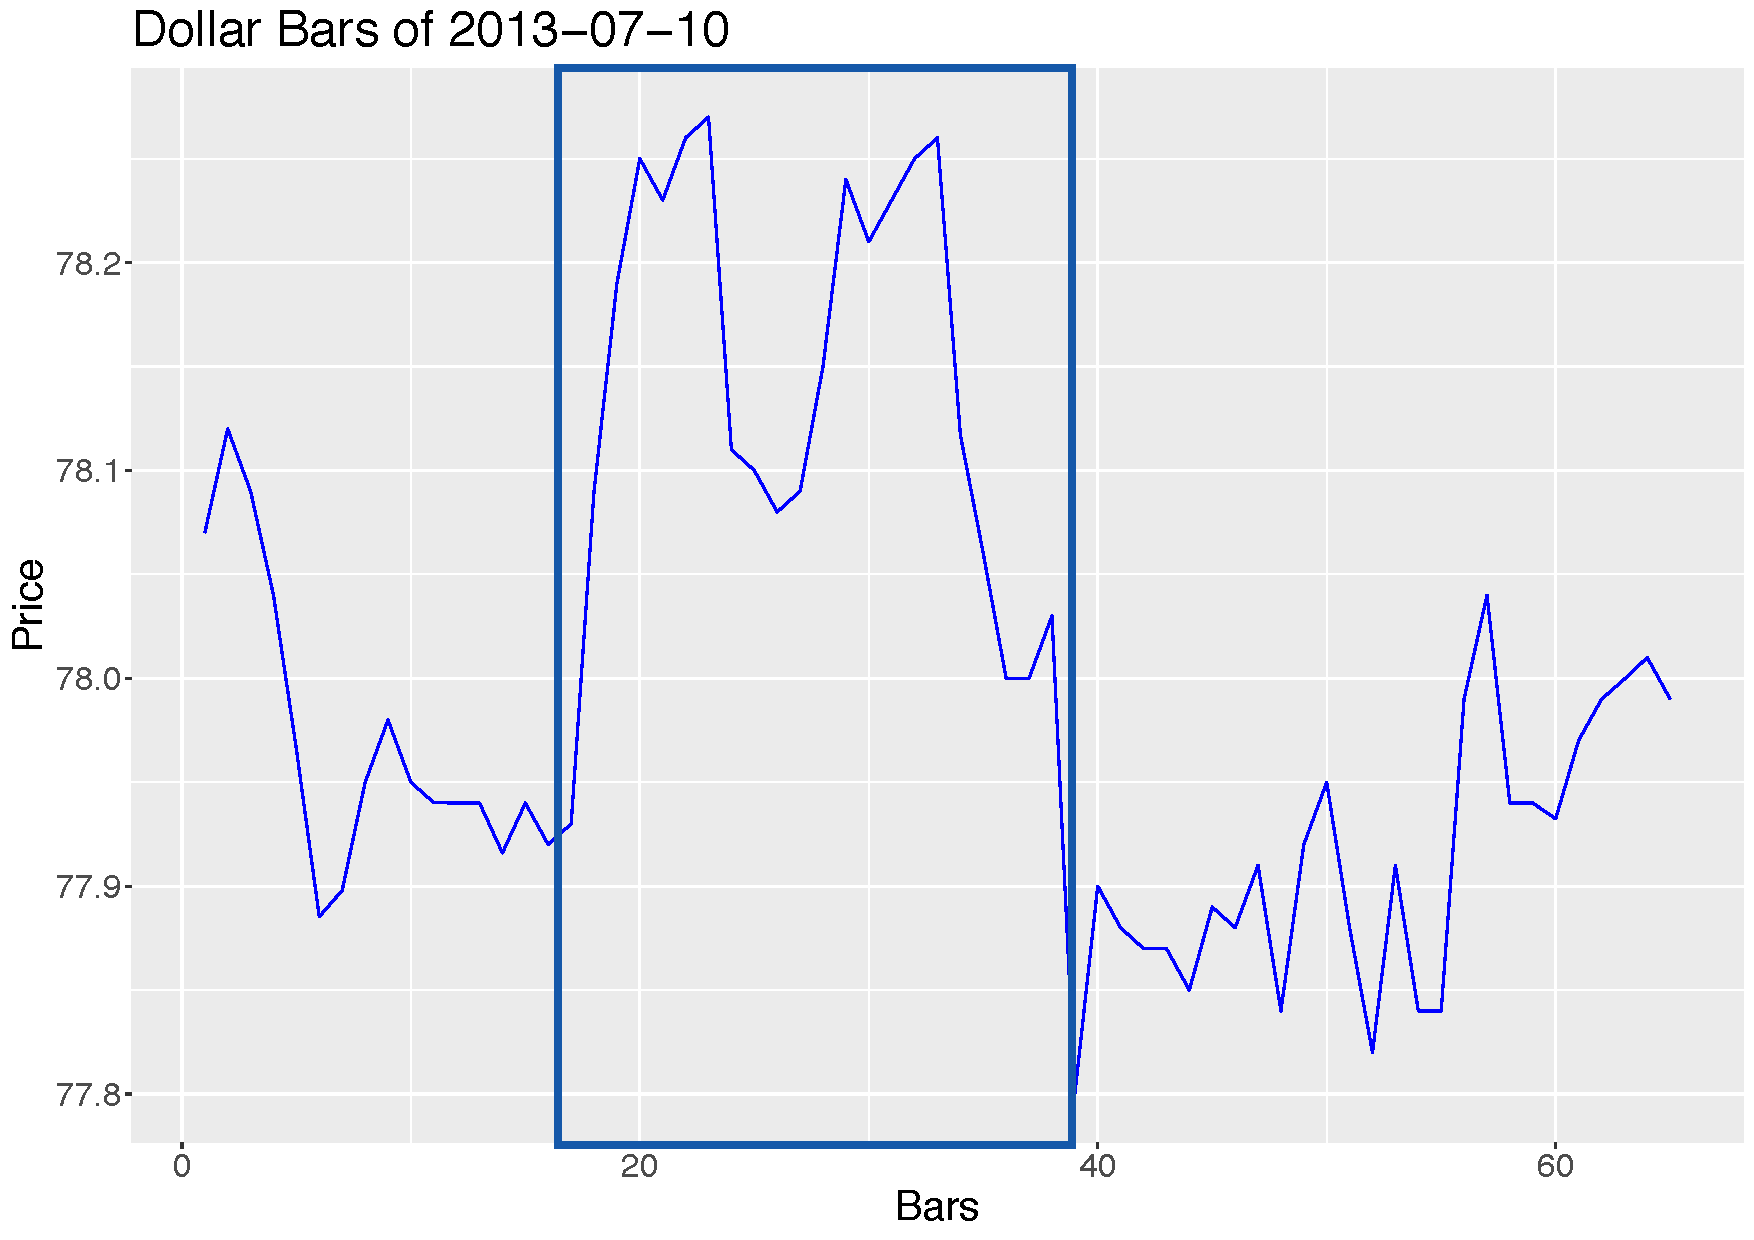
\includegraphics[scale=.15]{img/dollarZoomBis}
		\caption{Dollar bars}
	\end{subfigure}%
	\begin{subfigure}{.5\textwidth}
		\centering
		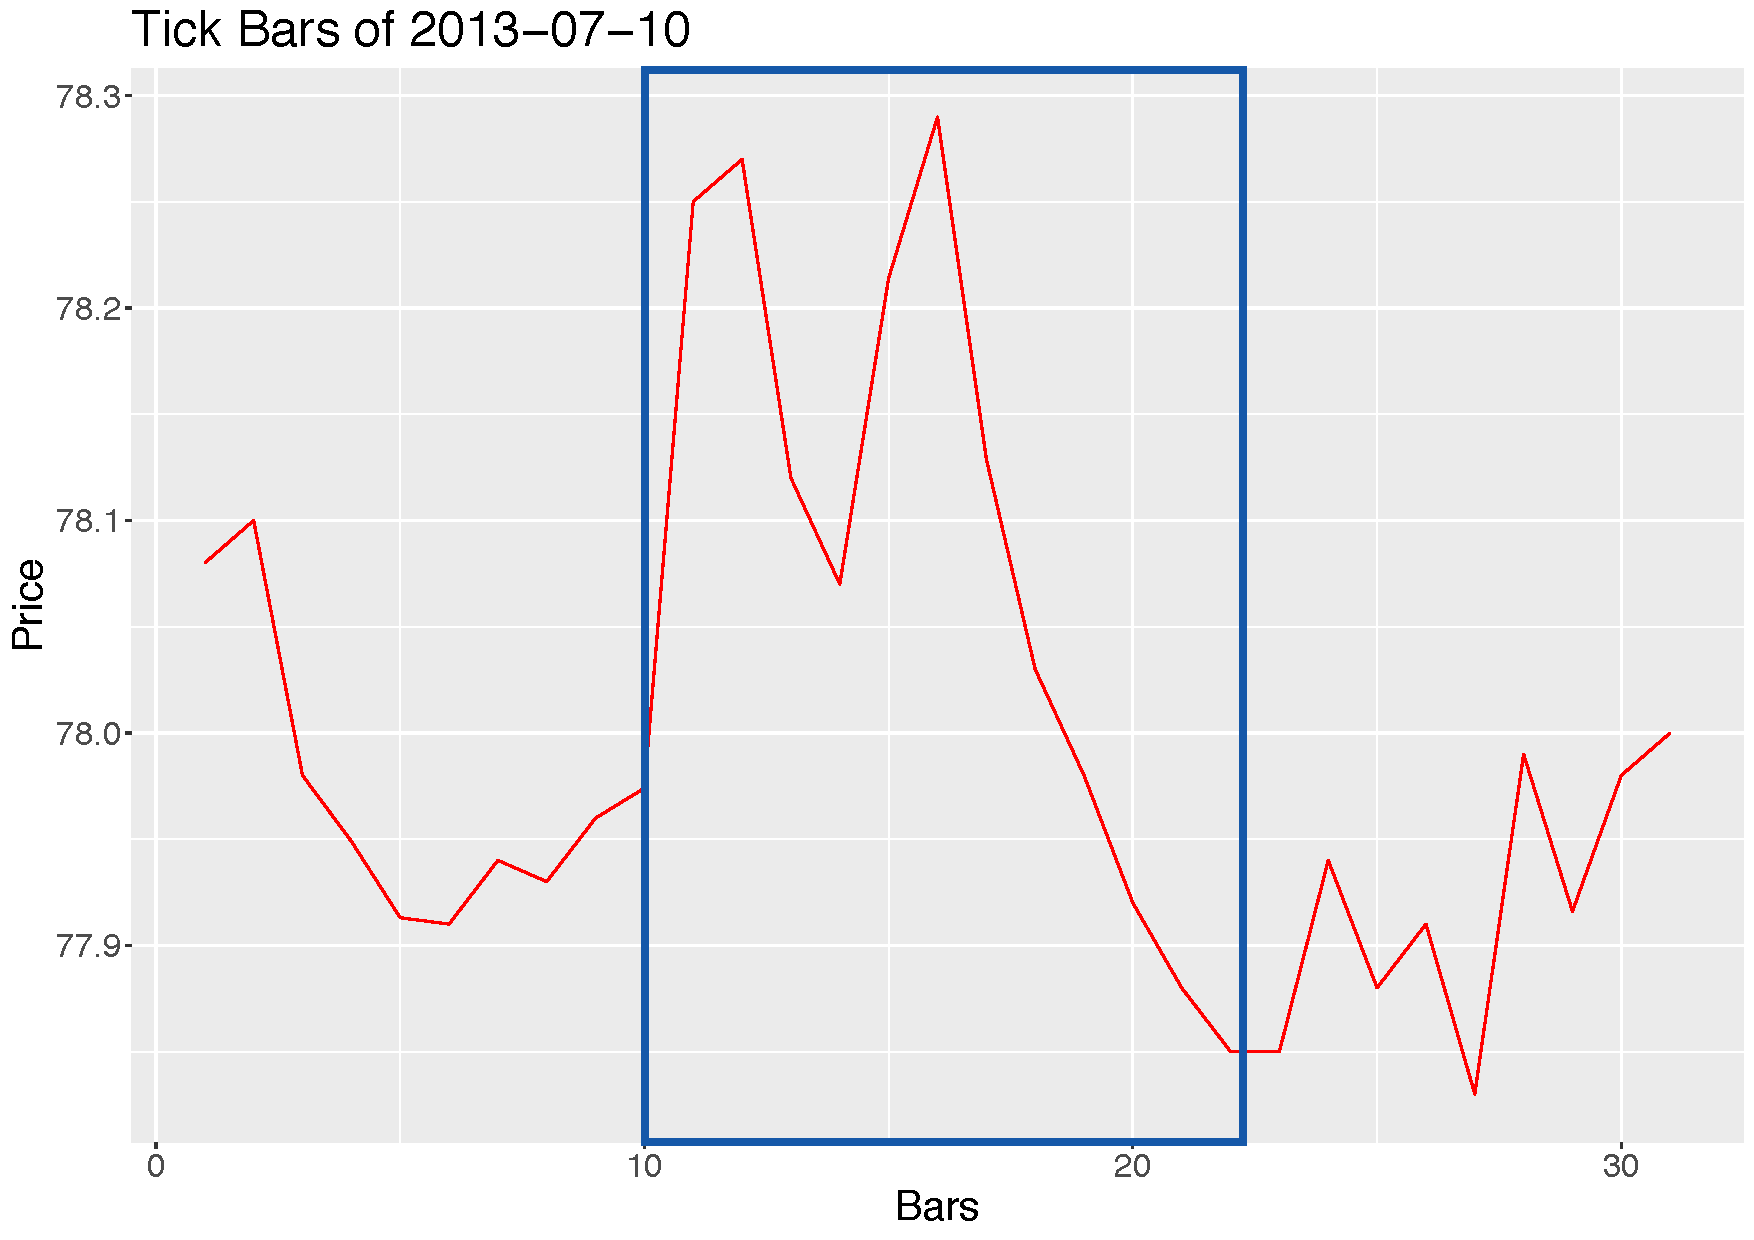
\includegraphics[scale=.15]{img/tickZoomBis}
		\caption{Tick bars}
	\end{subfigure}%
	
	%\caption{Sampling of 2013-07-10 tick data via tick, volume, dollar and 
	%time bars}
\end{figure}
\end{frame}

\begin{frame}{Models}
\vfill
When the different samples have been gathered, \textbf{log-returns will be 
computed for every type of bar}. Then, every type of bar will be 
\textbf{fitted an Autoregressive model} - AR($p$):

\vfill
\begin{equation*}
	r_k = c + \sum_{i=1}^p \theta_i r_{k-i} + \epsilon_k
\end{equation*}

\vfill
Note that \textbf{time bars} will be the \textbf{benchmark}, since these bars 
are the predominant sampling technique.

\begin{table}
\centering
\scalebox{0.9}{
\begin{tabular}{ |C{3cm}|C{2cm}|C{2cm}|C{2cm}|C{2cm}| }
	\hline
	 				& Time & Volume & Dollar & Tick\\
	\hline
	Lag ($p$) & 2 & 1 & 10 & 0\\
	MAPE & 2.041 & 1.130 & 1.134 & 1.188\\
	Improvement & 0\% & 44.64\% & 44.43\% & 41.82\%\\
	\hline
\end{tabular}
}
\end{table}
\end{frame}

\section{Conclusions}
\frame{\tableofcontents[currentsection]}

\begin{frame}{Conclusions and future work}
\textbf{Conclusions:}
\begin{itemize}
	\item Efficient market (daily data) $\Rightarrow$ Noise $\Rightarrow$ 
	``Garbage in, garbage out''
	
	\vspace{.15cm}
	\item Low signal-to-noise ratio.	
	
	\vspace{.15cm}
	\item These techniques are not plug-and-play solutions. In fact, we are 
	not	dealing with a matter of what, but when.
\end{itemize}

\vspace{.5cm}
\textbf{Future work:}
\begin{itemize}
	\item Develop ML models that take into account alternative financial 
	data.
	
	\vspace{.15cm}
	\item Explore High Frequency Trading strategies.
\end{itemize}

\end{frame}

\section{}
\begin{frame}
	\Large
	\begin{center}
		\textbf{Thank you for your attention}
		% Thank you for your attention	
	\end{center}

\end{frame}

\end{document}
